%!TEX root = ../Appendix.tex

\clearpage{}
\section{Result Size}
\label{s:ResultSize}

As with any fusion system, we must be careful that the size of the result code does not become too large when more and more processes are fused together. 

\subsection{Fusing Pipelines of Processes}
The following figure shows the maximum number of output states in the result when a particular number of processes are fused together in a pipelined-manner.

\smallskip
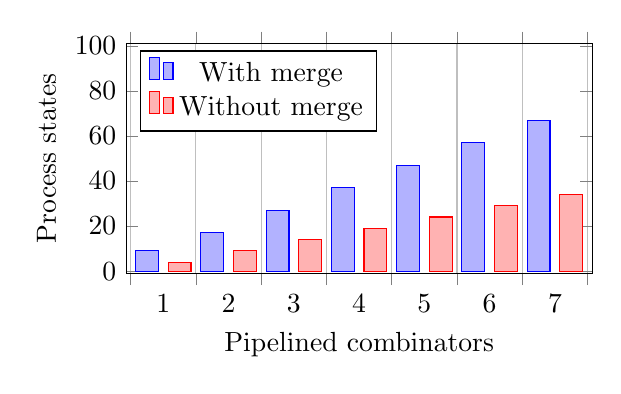
\begin{tikzpicture}
\begin{axis}[
% Hide the label on the second graph
        ylabel=Process states,
        xlabel=Pipelined combinators,
  ymin=0, ymax=100,
        enlargelimits=0.01,
        ybar interval=0.7,
  width=7.5cm, height=4.5cm,
        legend pos=north west,
]
\addplot coordinates {(1,9) (2,17) (3,27) (4,37) (5,47) (6,57) (7,67)   (8,1) };
\addplot coordinates {(1,4) (2,9) (3,14) (4,19) (5,24) (6,29) (7,34)    (8,1) };
\legend{With merge, Without merge};
\end{axis}
\end{tikzpicture}


To produce the above graph we programmatically generated dataflow networks for \emph{all possible} pipelined combinations of the @map@, @filter@, @scan@, @group@ and @merge@ combinators, and tried all possible fusion orders consiting of adjacent pairs of processes. The @merge@ combinator itself has two inputs, so only works at the very start of the pipeline --- we present result for pipelines with and without a @merge@ at the start. 

\subsection{Fusing Parallel Processes}
The following figure shows the number of states in the result when the various combinations of combinators are fused in parallel, for example, we might have a @map@ and a @filter@ processing the same input stream. In both cases the number of states in the result process grows linearly with the number of processes. In all combinations, with up to 7 processes there are less than 100 states in the result process.

\smallskip
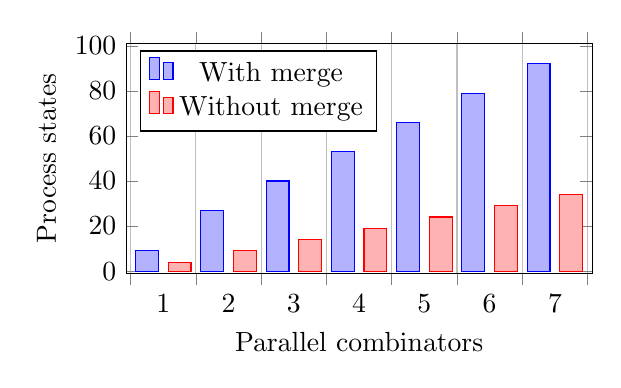
\begin{tikzpicture}
\begin{axis}[
        ylabel=Process states,
        xlabel=Parallel combinators,
  ymin=0, ymax=100,
        enlargelimits=0.01,
        ybar interval=0.7,
  width=7.5cm, height=4.5cm,
        legend pos=north west,
]
\addplot coordinates {(1,9) (2,27) (3,40) (4,53) (5,66) (6,79) (7,92)
  % Last bar doesn't show for some reason, so need to add a dummy value for the next one
    (8,1) };

\addplot coordinates {(1,4) (2,9) (3,14) (4,19) (5,24) (6,29) (7,34)    (8,1) };

\legend{With merge, Without merge};
\end{axis}
\end{tikzpicture}

The size of the result process is roughly what one would get when inlining the definitions of each of the original source processes. This is common with other systems based on inlining and/or template meta-programming, and is not prohibitive.


\eject{}
% -----------------------------------------------------------------------------
\subsection{Fusing Merges}

On the other hand, the following figure shows the results for a pathological case where the size of the output program is exponential in the number of input processes. The source dataflow networks consists of N merge processes, N+1 input streams, and a single output stream. The output of each merge process is the input of the next, forming a chain of merges. In source notation the network for N = 3 is @sOut = merge sIn1 (merge sIn2 (merge sIn3 sIn4))@.

\medskip
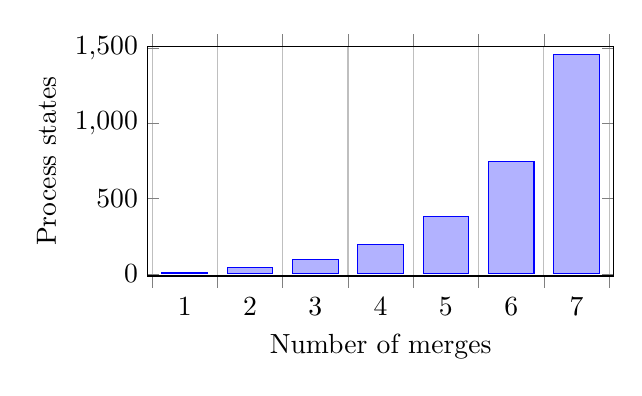
\begin{tikzpicture}
\begin{axis}[
        ylabel=Process states,
        xlabel=Number of merges,
%  ymode=log,
  ymin=0, ymax=1500,
        enlargelimits=0.01,
        ybar interval=0.7,
  width=7.5cm, height=4.5cm,
        legend pos=north west,
]
% These are the values for splitting.
% They are smaller than the 'chaining', but look much nicer on the linear graph.
\addplot coordinates {(1,9) (2,42) (3,97) (4,196) (5,383) (6,746) (7,1461)
  % (8,2880)
  (8,1)
  };

% These are the values for chaining
% \addplot coordinates {(1,4) (2,48) (3,194) (4,760) (5,2814) (6,10064) (7,1) };

\end{axis}
\end{tikzpicture}


When fusing two processes the fusion algorithm essentially compares every state in the first process with every state in the second, computing a cross product. During the fusion transform, as states in the result process are generated they are added to a finite map --- the @instrs@ field of the process definition. The use of the finite map ensures that identical states are always combined, but genuinely different states always make it into the result. 
In the worst case, fusion of two processes produces O($n*m$) different states, where $n$ and $m$ are the number of states in each. If we assume the two processes have about the same number of states then this is O($n^2$). Fusing the next process into this result yields O($n^3$), so overall the worst case number of states in the result will be O($n^k$), where $k$ is the number of processes fused. 

In the particular case of @merge@, the implementation has two occurrences of the @push@ instruction. During fusion, the states for the consuming process are inlined at each occurrence of @push@. These states are legitimately different because at each occurence of @push@ the input channels of the merge process are in different channel states, and these channel states are included in the overall process state.

